\chapter{Multipier et diviser avec les relatifs}\label{ChMultDivRelatifs}

\vspace{5cm}

\begin{acquis}
\begin{itemize}
\item multiplier deux nombres relatifs;
\item multiplier plus de deux nombres relatifs;
\item calculer des puissances de nombres relatifs;
\item diviser deux nombres relatifs;
\item faire des calculs contenant les 4 opérations et des parenthèses en respectant les priorités.
\end{itemize}
\end{acquis}


\activites

\begin{activite}[Produit d'un nombre négatif par un nombre positif] \label{MultDivRelatifs_acti1}

On considère l'expression $A = (-2) + (-2) + (-2) + (-2)$.

\begin{partie}
Quelle est la valeur de $A$ ? \\[0.5em]
On va revenir sur le sens de la multiplication : $20 + 20 + 20$ est la somme de trois termes tous égaux. On peut donc écrire cette somme sous la forme du produit $20 \times 3$ qui se lit « 20 multiplié par 3 ».
\end{partie}

\begin{partie}
Écris $A$ sous la forme d'un produit.
 \end{partie}
 
\begin{partie} 
Écris les expressions suivantes sous la forme d'une somme et calcule-les :
 \begin{colenumerate}{4}
  \item $(-6) \times 3$ ;
  \item $(-22) \times 5$ ;
  \item $(-7) \times 7$ ;
  \item $(-1,5) \times 6$.
  \end{colenumerate}
 \end{partie}
 
\begin{partie} \label{MultDivRelatifs_acti2}
Trouve une règle permettant de calculer le produit d'un nombre négatif par un nombre positif.
 \end{partie}

\end{activite}

%%%%%%%%%%%%%%%%%%%%%%%%%%%%%%%%%%%%%%%%%%%%%%%%%%%%%%%%%%%%%%%%%%%%%%%%%

\begin{activite}[À propos des produits]

\begin{minipage}[c]{0.66\linewidth}
\begin{partie}
Voici une table de multiplication :
\begin{enumerate}
 \item Recopie-la sur ton cahier et complète la partie qui concerne le produit de deux nombres positifs (en bas à droite).
 \item D'après le résultat de la partie \ref{MultDivRelatifs_acti2} de l'activité \ref{MultDivRelatifs_acti1}, complète la partie qui concerne le produit d'un nombre négatif par un nombre positif (en haut à droite).
 \item Observe les résultats dans cette table de multiplication et complète-la entièrement, en expliquant tes choix.
 \item À l'aide d'un tableur, crée cette table de multiplication et vérifie que les résultats obtenus sont les mêmes que les tiens.
 \end{enumerate}
\end{partie}
\end{minipage} \hfill%
 \begin{minipage}[c]{0.3\linewidth}
  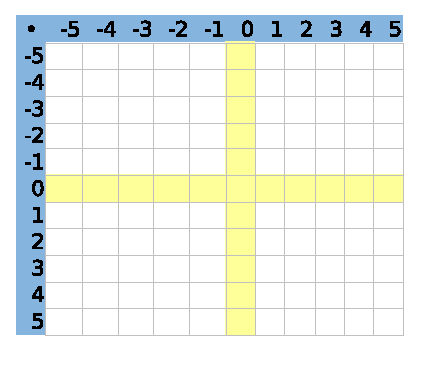
\includegraphics[width=5cm]{grille_produits}
  \end{minipage} \\

\begin{partie}
Application sur quelques exemples :
\begin{enumerate}
 \item En t'aidant de la table, donne le résultat pour chaque calcul suivant :
 \begin{colitemize}{4}
  \item $A = (-5) \times 4$ ;
  \item $B = 3 \times (-2)$ ;
  \item $C = 5 \times (-4)$ ;
  \item $D = (-1) \times (-3)$.
  \end{colitemize}
 \item En t'inspirant de ce qui précède, propose un résultat pour les calculs suivants :
 \begin{colitemize}{4}
  \item $E = (-9,2) \times 2$ ;
  \item $F = 1,5 \times (-8)$ ;
  \item $G = (-3,14) \times 0$ ;
  \item $H = (-1,2) \times (-0,1)$.
  \end{colitemize}
 \item Vérifie ces résultats à la calculatrice.
 \end{enumerate}
\end{partie}

\begin{partie}
Propose une règle qui permet, dans tous les cas, de calculer le produit de deux nombres relatifs.
\end{partie}

\end{activite}

%%%%%%%%%%%%%%%%%%%%%%%%%%%%%%%%%%%%%%%%%%%%%%%%%%%%%%%%%%%%%%%%%%%%%%%%%

\begin{activite}[Produit de plusieurs nombres relatifs]

\begin{partie}
Calcule ces expressions et déduis-en une règle pour trouver rapidement chaque résultat :
\begin{itemize}
 \item $A = (-1) \times (-1)$ ;
 \item $B = (-1) \times (-1) \times (-1)$ ;
 \item $C = (-1) \times (-1) \times (-1) \times (-1)$ ;
 \item $D = (-1) \times (-1) \times (-1) \times (-1) \times (-1)$ ;
 \item $E = (-1) \times (-1) \times (-1) \times (-1) \times (-1) \times (-1)$.
 \end{itemize}
\end{partie}

\begin{partie}
On sait que $(-4) = (-1) \times 4$ et $(-2) = (-1) \times 2$.
\begin{enumerate}
 \item Complète alors le calcul suivant :
\begin{center} $(-4) \times (-2) \times (-5) = (-1) \times \ldots \times (-1) \times \ldots \times (- ) \times \ldots$ \end{center}
\begin{center} $\phantom{(-4) \times (-2) \times (-5) }= (-1) \times (-1) \times (-1) \times \ldots \times \ldots \times \ldots$ \end{center}
 \item Déduis-en une méthode pour trouver le résultat de $(-4) \times (-2) \times (-5)$.
 \end{enumerate}
\end{partie}

\begin{partie}
Inspire-toi de la question précédente pour effectuer le calcul suivant :
\begin{itemize}
 \item $F = (-2) \times (-3) \times 5 \times (-4) \times 6 \times (-5)$.
 \end{itemize}
\end{partie}

\begin{partie}
Propose une méthode pour multiplier plusieurs nombres relatifs.
\end{partie}

\end{activite}

%%%%%%%%%%%%%%%%%%%%%%%%%%%%%%%%%%%%%%%%%%%%%%%%%%%%%%%%%%%%%%%%%%%%%%%%%

\begin{activite}[Quotient de nombres relatifs]

Revenons sur le sens de la division : \\[0.5em]
Écrire $3 \times 5 = 15$ revient à écrire $3 = 15 : 5$ ou $5 = 15 : 3$.
       
\begin{partie}
Recopie et complète les trous par les nombres manquants pour que les égalités soient correctes :
\begin{colenumerate}{4}
 \item $4 \times  \ldots = 12$ ;
 \item $(-5) \times  \ldots = 130$ ;
 \item $8 \times  \ldots = (-16)$ ;
 \item $ \ldots \times (-3) = (-27)$.
 \end{colenumerate}
\end{partie}

\begin{partie}
Écris ces nombres manquants sous forme de quotients.
\end{partie}

\begin{partie}
Que dire du quotient de deux nombres relatifs ?
\end{partie}

\end{activite}

%%%%%%%%%%%%%%%%%%%%%%%%%%%%%%%%%%%%%%%%%%%%%%%%%%%%%%%%%%%%%%%%%%%%%%%%%


\cours
%\section{Une section}

% remarque : pour qu'un mot se retrouve dans le lexique : \MotDefinition{asymptote horizontale}{} 

\begin{aconnaitre}
Pour multiplier deux nombres relatifs, on multiplie les valeurs absolues et on applique la \MotDefinition{règle des signes}{} :
\begin{itemize}
 \item Le produit de deux nombres relatifs de \textbf{même signe} est \textbf{positif} ;
 \item Le produit de deux nombres relatifs de \textbf{signes opposés} est \textbf{négatif}.
 \end{itemize}
\end{aconnaitre}

\begin{methode*1}[Multiplier deux nombres relatifs]

 \begin{exemple*1}
Effectue la multiplication : $E = (-4) \times (-2,5)$. \\[0.5em]
Le résultat est positif car c'est le produit de deux nombres négatifs :

$E = 4 \times 2,5$, \hspace{3cm} $E = 10$.
 \end{exemple*1}

 \begin{exemple*1}
Effectue la multiplication : $F = 0,2 \times (-14)$. \\[0.5em]
Le résultat est négatif car c'est le produit d'un nombre positif par un nombre négatif :

$F = -(0,2 \times 14)$, \hspace{3cm}

$F = -2,8$.
 \end{exemple*1}

 \exercice  
Effectue les multiplications suivantes :
\vspace{1em}
\begin{colenumerate}{3}
 \item $(-7) \times (-8)$ \dotfill;
 \vspace{1em}
 \item $-5 \times (-11)$ \dotfill;
 \vspace{1em}
 \item $(-9) \times 6$ \dotfill;
 \vspace{1em}
 \item $-8 \times 0,5$ \dotfill;
 \vspace{1em}
 \item $10 \times (-0,8)$ \dotfill;
 \vspace{1em}
 \item $(-7) \times 0$\dotfill.
 \end{colenumerate}
%\correction



 \end{methode*1}
 
 %%%%%%%%%%%%%%%%%%%%%%%%%%%%%%%%%%%%%%%%%%%%%%%%%%%%%%%%%%%%%%%%%%%%%%%%
 %%%%%%%%%%%%%%%%%%%%%%%%%%%%%%%%%%%
%%%%%%%%%%%%%%%%%%%%%%%%%%%%%%%%%%%
%MiseEnPage
%%%%%%%%%%%%%%%%%%%%%%%%%%%%%%%%%%%
\vspace{2cm}
%%%%%%%%%%%%%%%%%%%%%%%%%%%%%%%%%%%
%%%%%%%%%%%%%%%%%%%%%%%%%%%%%%%%%%%
 
 
 \begin{aconnaitre}
 \begin{itemize}
  \item Le produit de plusieurs nombres relatifs est \textbf{positif} s'il comporte un nombre \textbf{pair} de \textbf{facteurs négatifs} ;
  \item Le produit de plusieurs nombres relatifs est \textbf{négatif} s'il comporte un nombre \textbf{impair} de \textbf{facteurs négatifs}.
  \end{itemize}
\end{aconnaitre}

%%%%%%%%%%%%%%%%%%%%%%%%%%%%%%%%%%%
%%%%%%%%%%%%%%%%%%%%%%%%%%%%%%%%%%%
%MiseEnPage
%%%%%%%%%%%%%%%%%%%%%%%%%%%%%%%%%%%
\newpage
%%%%%%%%%%%%%%%%%%%%%%%%%%%%%%%%%%%
%%%%%%%%%%%%%%%%%%%%%%%%%%%%%%%%%%%

\begin{methode*1}[Multiplier plusieurs nombres relatifs]

 \begin{exemple*1}
Quel est le signe du produit : $A = -6 \times 7 \times (-8) \times (-9)$ ? \\[0.5em]
Le produit a trois facteurs négatifs. 3 est impair donc $A$ est négatif.
 \end{exemple*1}
 
  \begin{exemple*1}
Calcule le produit : $B = 2 \times (-4) \times (-5) \times (-2,5) \times (-0,8)$. \\[0.5em]
Il y a quatre facteurs négatifs; 4 est pair donc $B$ est positif : \\
$B = 2 \times 4 \times 5 \times 2,5 \times 0,8$ ; \hspace{1cm}  $B = (2 \times 5) \times (4 \times 2,5) \times 0,8$ ; \\       
$B = 10 \times 10 \times 0,8$ ; \hspace{1cm} $B = 80$.
 \end{exemple*1}
 
 \exercice  
Quel est le signe du produit $C = 9 \times (-9) \times (-9) \times 9 \times (-9) \times (-9) \times (-9)$ ?
%\correction
     
 \exercice  
Calcule :
\vspace{.5em}
\begin{colenumerate}{2}
 \item $-25 \times (-9) \times (-4)$ \dotfill;
 \item $0,5 \times 6 \times (-20) \times 8$ \dotfill.
 \end{colenumerate}
 %\correction

 \end{methode*1}
 
 %%%%%%%%%%%%%%%%%%%%%%%%%%%%%%%%%%%%%%%%%%%%%%%%%%%%%%%%%%%%%%%%%%%%%%%%
 
 \begin{aconnaitre}
Pour diviser deux nombres relatifs non nuls, on divise les valeurs absolues et on applique la \MotDefinition{règle des signes}{} :
\begin{itemize}
 \item Le quotient de deux nombres relatifs de \textbf{même signe} est \textbf{positif} ;
 \item Le quotient de deux nombres relatifs de \textbf{signes opposés} est \textbf{négatif}.
 \end{itemize}
\end{aconnaitre}

\begin{methode*1}[Diviser deux nombres relatifs]

 \begin{exemple*1}
Effectue la division suivante : $A = 65 : (-5)$. \\[0.5em]
Le résultat est négatif car c'est le quotient de deux nombres de signes opposés :

$65 : 5 = 13$ donc $A = -13$.
 \end{exemple*1}
 
 
 \begin{exemple*1}
Effectue la division: $B = (-30) : (-4)$. \\[0.5em]
Le résultat est positif car c'est le quotient de deux nombres négatifs :

$B = 30 : 4$,

$B = 7,5$.
 \end{exemple*1}
 
 \exercice  
Quel est le signe des quotients suivants ?
\vspace{1em}
\begin{colenumerate}{4}
 \item $56 : (-74)$ \dotfill;
 \item $(-6) : (-5)$ \dotfill;
 \item $9 : (-13)$ \dotfill;
 \item $-7 : (-45)$\dotfill.
 \end{colenumerate}
%\correction

 \exercice  
Calcule de tête :
\vspace{1em}
\begin{colenumerate}{4}
 \item $45 : (-5)$\dotfill;
 \item $(-56) : (- 8)$ \dotfill;
 \item $-59 : (-10)$ \dotfill;
 \item $-14 : 4$\dotfill.
 \end{colenumerate}
%\correction

 \end{methode*1}
 
 %%%%%%%%%%%%%%%%%%%%%%%%%%%%%%%%%%%%%%%%%%%%%%%%%%%%%%%%%%%%%%%%%%%%%%%%


\exercicesbase
\begin{colonne*exercice}

\serie{Produits de relatifs}

\begin{exercice}
Complète : 
\begin{enumerate}
 \item $A = (-4) + (-4) + (-4) + (-4) + (-4)$
 
$A = (-4) \times \ldots \ldots$

$A = \ldots \ldots$
 \item $B = (-8,2) + (-8,2) + (-8,2)$
 
$B = (-8,2) \times \ldots \ldots$

$B = \ldots \ldots$
 \item $C = (-1,7) + (-1,7) + (-1,7) + (-1,7)$

$C = (-1,7) \times \ldots \ldots$

$C = \ldots \ldots$
 \end{enumerate}
\end{exercice}


\begin{exercice}
Sans les calculer, donne le signe de chacun des produits suivants :
\begin{colenumerate}{2}
 \item $(-12) \times (+2)$ \dotfill;
 \item $(+34) \times (-28)$ \dotfill;
 \item $(-10,3) \times (-46)$ \dotfill;
 \item $(+12,5) \times (+3,1)$\dotfill.
 \end{colenumerate}
\end{exercice}


\begin{exercice}
Sans les calculer, donne le signe de chacun des produits suivants :
\begin{colenumerate}{2}
 \item $-36 \times (-1)$ \dotfill;
 \item $(-2) \times (+24)$ \dotfill; 
 \item $2,3 \times (-2,3)$ \dotfill;
 \item $-9,1 \times 6$\dotfill.
 \end{colenumerate}
\end{exercice}


\begin{exercice}
Quel est le signe du résultat quand on :
\begin{enumerate}
 \item multiplie un nombre négatif par un nombre positif ? \ldots \ldots
 \item multiplie quatre nombres négatifs entre eux ?  \ldots \ldots
 \item multiplie un nombre positif et deux nombres négatifs ?  \ldots \ldots
 \item multiplie un nombre relatif par lui-même ? \ldots \ldots
 \item multiplie trois nombres négatifs entre eux ? \ldots \ldots
 \end{enumerate}
\end{exercice}


\begin{exercice}
Effectue :
\begin{colenumerate}{2}
 \item $(+5) \times (-4)$ \dotfill;
 \item $(-5) \times (-3)$ \dotfill;
 \item $(-3) \times (+4)$ \dotfill;
 \item $(+4) \times (+4)$ \dotfill;
 \item $(-4) \times (-3)$ \dotfill;
 \item $(-5) \times (-4)$ \dotfill;
 \item $(-5) \times (+3)$ \dotfill;
 \item $(-4) \times (+4)$\dotfill.
 \end{colenumerate}
\end{exercice}


\begin{exercice}
Effectue :
\begin{colenumerate}{2}
 \item $(-8) \times (+2)$ \dotfill;
 \item $(-2) \times (+5) $ \dotfill;
 \item $(-4) \times (-8)$ \dotfill;
 \item $(+9) \times (+10)$ \dotfill; 
 \item $(+191) \times (+0,1)$ \dotfill; 
 \item $(-1,5) \times (+20)$ \dotfill;
 \item $(-0,25) \times (-4)$ \dotfill;
 \item $(+0,8) \times (-3)$ \dotfill;
 \item $(-3,2) \times (+4)$ \dotfill;
 \item \phantom{.} $(-1) \times (-17)$\dotfill.
 \end{colenumerate}
\end{exercice}


\begin{exercice}
Calcule, sachant que $11,2 \times 2,5 = 28$ :
\begin{colenumerate}{2}
 \item $11,2 \times (-2,5)$  \dotfill;
 \item $-11,2 \times (-2,5)$ \dotfill.
 \end{colenumerate}
\end{exercice}

%%%%%%%%%%%%%%%%%%%%%%%%%%%%%%%%%%%
%%%%%%%%%%%%%%%%%%%%%%%%%%%%%%%%%%%
%MiseEnPage
%%%%%%%%%%%%%%%%%%%%%%%%%%%%%%%%%%%
\columnbreak
%%%%%%%%%%%%%%%%%%%%%%%%%%%%%%%%%%%
%%%%%%%%%%%%%%%%%%%%%%%%%%%%%%%%%%%

\begin{exercice}
\emph{Un produit peut en cacher un autre \ldots}
\begin{enumerate}
 \item Calcule le produit $7,5 \times 0,2$ \dotfill ;
 \item Effectue alors les calculs suivants :
 \begin{colitemize}{1}
  \item $A=7,5\times(-0,2)$ \dotfill;
  \item $B=(-0,2)\times(-7,5)$ \dotfill;
  \item $C=(-75)\times(+0,2)$ \dotfill;
  \item $D=(-7,5)\times(-20)$\dotfill.
  \end{colitemize}
 \end{enumerate}
\end{exercice}


\begin{exercice}
Relie les expressions dont les produits sont égaux :
\begin{center}
 \begin{tabularx}{\linewidth}{|c|cXc|c|}
  \cline{1-1}\cline{5-5}
  \cellcolor{F3} $(+5) \times (-12)$ & \cellcolor{F2} $\bullet$ & & \cellcolor{F2} $\bullet$ & \cellcolor{F3} $(-1) \times (+20)$ \\  \cline{1-1}\cline{5-5}
  \cellcolor{F3} $(-8) \times (-3)$ & \cellcolor{F2} $\bullet$ & & \cellcolor{F2} $\bullet$ & \cellcolor{F3} $(+12) \times (+5)$ \\ \cline{1-1}\cline{5-5}
  \cellcolor{F3} $(+4) \times (-6)$ & \cellcolor{F2} $\bullet$ & & \cellcolor{F2} $\bullet$ & \cellcolor{F3} $(+2) \times (+12)$ \\ \cline{1-1}\cline{5-5}
  \cellcolor{F3} $(+5) \times (-4)$ & \cellcolor{F2} $\bullet$ & & \cellcolor{F2} $\bullet$ & \cellcolor{F3} $(+5) \times (+4)$ \\ \cline{1-1}\cline{5-5}
  \cellcolor{F3} $(+2) \times (+10)$ & \cellcolor{F2} $\bullet$ & & \cellcolor{F2} $\bullet$ & \cellcolor{F3} $(-3) \times (+20)$ \\ \cline{1-1}\cline{5-5}
  \cellcolor{F3} $(-2) \times (-30)$ & \cellcolor{F2} $\bullet$ & & \cellcolor{F2} $\bullet$ & \cellcolor{F3} $(-12) \times (+2)$ \\ \cline{1-1}\cline{5-5}
  \end{tabularx}
\end{center}
\end{exercice}


\begin{exercice}
Complète la table de multiplication suivante :
\begin{center}
 \renewcommand*\tabularxcolumn[1]{>{\centering\arraybackslash}m{#1}}
 \begin{ttableau}{\linewidth}{6}
  \hline
  \rowcolor{A2} $\times$ & $-3$ & $+5$ & $-9$ & $+6$ & $-8$ \\\hline
  \cellcolor{A2} $-1$ & \cellcolor{A3} & \cellcolor{A3} & \cellcolor{A3} & \cellcolor{A3} & \cellcolor{A3} \\\hline
  \cellcolor{A2} $+4$ & \cellcolor{A3} & \cellcolor{A3} & \cellcolor{A3} & \cellcolor{A3} & \cellcolor{A3} \\\hline
  \cellcolor{A2} $-7$ & \cellcolor{A3} & \cellcolor{A3} & \cellcolor{A3} & \cellcolor{A3} & \cellcolor{A3} \\\hline
  \cellcolor{A2} $0$ & \cellcolor{A3} & \cellcolor{A3} & \cellcolor{A3} & \cellcolor{A3} & \cellcolor{A3} \\\hline
  \end{ttableau}
\end{center}
\end{exercice}


\begin{exercice}
Complète les « pyramides » sachant que le nombre contenu dans une case est le produit des nombres contenus dans les deux cases situées en dessous de lui : \\[0.3em]
\begin{minipage}[c]{0.48\linewidth}
\begin{center} 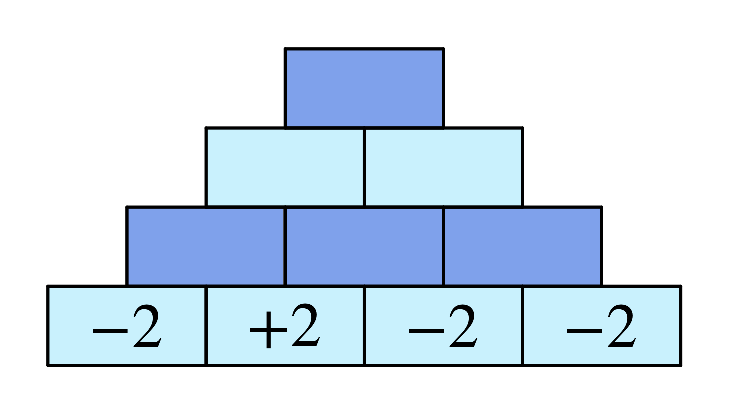
\includegraphics[width=4cm]{pyramide1_MultDivRelatifs} \end{center}
\end{minipage} \hfill%
 \begin{minipage}[c]{0.48\linewidth}
\begin{center} 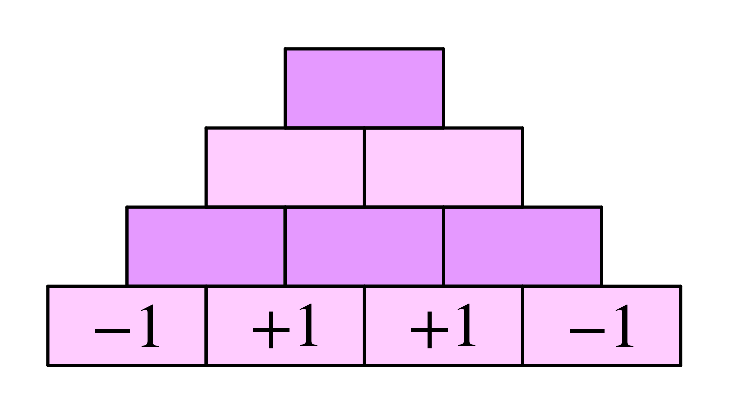
\includegraphics[width=4cm]{pyramide2_MultDivRelatifs} \end{center}  
\end{minipage} \\

\end{exercice}


\begin{exercice}
Donne le signe de chacun des produits suivants :
\begin{enumerate}
 \item $5,4 \times (-3,2) \times (+4) \times (-5,1)$ \ldots \ldots;
 \item $(-0,5) \times (-9) \times 0 \times 7 \times (-1,4) \times (-1)$ \ldots \ldots;
 \item $-6 \times (-10) \times 4 \times (-9) \times (-3) \times (-4,1)$\ldots \ldots.
 \end{enumerate}
\end{exercice}


\begin{exercice}
Effectue les calculs suivants :
\begin{enumerate}
 \item $(-2) \times (-3) \times (+5)$ \dotfill;
 \item $(-3) \times (-2) \times (-4)$  \dotfill;
 \item $(+6) \times (-1) \times (+3)$ \dotfill.
 \end{enumerate}
\end{exercice}


\begin{exercice}
Effectue les calculs suivants :
\begin{enumerate}
 \item $(-3,2) \times (-10) \times (+2) \times (-0,5)$  \dotfill;
 \item $(-75) \times (-0,25) \times (+4) \times (+2)$  \dotfill;
 \item $(-3) \times (-0,1) \times (+5) \times (+4)$  \dotfill;
 \item $(-1,5) \times (+4) \times (-1) \times (+0,8) \times (-3)$  \dotfill;
 \item $(+2) \times (-10) \times (+3) \times (-1) \times (-1)$ \dotfill.
 \end{enumerate}
\end{exercice}


\begin{exercice}
Calcule astucieusement :
\begin{enumerate}
 \item $(-2) \times (-1,25) \times (-2,5) \times (-8)$  \dotfill;
 \item $(-75) \times (-0,25) \times (+2) \times (+4)$  \dotfill;
 \item $(+0,01) \times (-25) \times (-13,2) \times 4 \times (-3)$ \dotfill.
 \end{enumerate}
\end{exercice}


\begin{exercice}
Complète les pointillés par le nombre qui convient :
\begin{colenumerate}{2}
 \item $(-4) \times \ldots = 20$ ;
 \item $(-13) \times \ldots = -39$ ;  
 \item $\ldots \times 7 = -42$ ;
 \item $\ldots \times (-11) = 121$.
 \end{colenumerate}
\end{exercice}


\begin{exercice}
Complète les pointillés par le nombre qui convient :
\begin{colenumerate}{2}
 \item $(+4) \times \ldots = -100$ ;
 \item $(-2,9) \times \ldots = 29$ ;  
 \item $\ldots \times 17 = -17$ ;
 \item $\ldots \times (-3) = -99$.
 \end{colenumerate}
\end{exercice}


\begin{exercice}[Suite logique de nombres]
Donne le signe de chacun des produits suivants :
\begin{enumerate}
 \item $(-1) \times 2 \times (-3) \times 4 \times \ldots \times (-9)$ ;
 \item $(-1) \times (-2) \times (-3) \times (-4) \times \ldots \times (-12)$ ;
 \item $(-4) \times (-3) \times (-2) \times \ldots \times 3 \times 4 \times 5$ ;
 \item $5 \times (-10) \times 15 \times (-20) \times \ldots \times (-100)$ ;
 \item $1 \times (-2) \times 4 \times (-8) \times \ldots \times 1\,024$.
 \end{enumerate}
\end{exercice}


\begin{exercice}[Températures]
Il fait $0^\circ$C et la température chute de deux degrés toutes les heures. 
\begin{enumerate}
 \item Combien de temps faudra-t-il pour que la température atteigne $-10^\circ$C ?
 \item Quelle sera la température dans huit heures ?
 \end{enumerate}
\end{exercice}


\begin{exercice}
Calcule dans chaque cas le produit $x \times y$ :
\begin{colenumerate}{2}
 \item $x = 5$ et $y = -3$ ;
 \item $x = +4$ et $y = -11$ ;
 \item $x = -2$ et $y = -5$ ;
 \item $x = -0,5$ et $y = -5,2$.
 \end{colenumerate}
\end{exercice}


\begin{exercice}
Complète le tableau suivant :
{\small
\begin{center}
\begin{tabular}{|c|c|c|c|c|c|c|}
\hline
\cellcolor{H2} $a$ & \cellcolor{H2} $b$ & \cellcolor{H2} $c$ & \cellcolor{A2} $ab$ &  \cellcolor{A2} ($-a$) $\cdot$ $c$ &  \cellcolor{A2} $-(a\cdot c)$ &  \cellcolor{A2} $a \cdot b \cdot c$ \\\hline 
\cellcolor{H3} $-5$ & \cellcolor{H3} $+6$ & \cellcolor{H3} $-4$ & \cellcolor{A3} & \cellcolor{A3} & \cellcolor{A3} & \cellcolor{A3} \\\hline
\cellcolor{H3} $-1$ & \cellcolor{H3} $-2$ & \cellcolor{H3} $-3$ & \cellcolor{A3} & \cellcolor{A3} & \cellcolor{A3} & \cellcolor{A3} \\\hline
\cellcolor{H3} $-2,1$ & \cellcolor{H3} $-4$ & \cellcolor{H3} $+3$ & \cellcolor{A3} & \cellcolor{A3} & \cellcolor{A3} & \cellcolor{A3} \\\hline
 \end{tabular}
 \end{center}
 } % fin du small
\end{exercice}


\begin{exercice}[Décompositions \ldots]
\begin{enumerate}
 \item Trouve toutes les façons de décomposer le nombre $-20$ en produit de deux nombres entiers relatifs.
 \item Trouve toutes les façons de décomposer le nombre 24 en produit de trois nombres entiers relatifs.
 \end{enumerate}
\end{exercice}


%%%%%%%%%%%%%%%%%%%%%%%%%%%%%%%%%%%
%%%%%%%%%%%%%%%%%%%%%%%%%%%%%%%%%%%
%MiseEnPage
%%%%%%%%%%%%%%%%%%%%%%%%%%%%%%%%%%%
\columnbreak
%%%%%%%%%%%%%%%%%%%%%%%%%%%%%%%%%%%
%%%%%%%%%%%%%%%%%%%%%%%%%%%%%%%%%%%

\begin{exercice}
Sans calculer, donne le signe de chaque résultat :
\begin{colenumerate}{3}
 \item $(-6)^{4}$   \dotfill;
 \item $6^{8}$  \dotfill;
 \item $-132^{51}$  \dotfill;
 \item $(-12)^{15}$  \dotfill;
 \item $(-3)^{7}$  \dotfill;
 \item $(-6)^{100}$  \dotfill;
 \item $-(-35)^{7}$  \dotfill;
 \item $-87^{4}$  \dotfill;
 \item $-(-13^{8})$ \dotfill.
 \end{colenumerate}
\end{exercice}


\begin{exercice}[Puissance de 1 ou de $-1$]
Calcule :
\begin{colenumerate}{4}
 \item $1^{12}$  \dotfill;
 \item $1^{0}$  \dotfill;
 \item $(-1)^{8}$  \dotfill;
 \item $(-1)^{0}$  \dotfill;
 \item $-1^{7}$  \dotfill;
 \item $-1^{6}$  \dotfill;
 \item $(-1)^{9}$  \dotfill;
 \item $-1^{0}$ \dotfill.
 \end{colenumerate}
\end{exercice}

%%%%%%%%%%%%%%%%%%%%%%%%%%%%%%%%%%%%%%%%%%%%%%%%%%%%%%%%%%%%%%%%%%%%%%%%%%%%%

\serie{Quotients de relatifs}

\begin{exercice}
Complète chaque égalité et écris chaque facteur manquant $\lozenge$ sous la forme d'un quotient :
\begin{enumerate}
 \item $(+6) \times \lozenge = +18$ donc $\lozenge = \ldots$ ;
 \item $(+5) \times \lozenge = -20$ donc $\lozenge = \ldots$ ;
 \item $\lozenge \times (-7) = +14$ donc  $\lozenge = \ldots$ ;
 \item $(-2) \times \lozenge = +12$ donc  $\lozenge = \ldots$ ;
 \item $\lozenge \times (-10) = -130$ donc  $\lozenge = \ldots$.
 \end{enumerate}
\end{exercice}


\begin{exercice}
Sans les calculer, donne le signe de chacun des quotients suivants :
\begin{colenumerate}{2}
 \item $(-3) \div (-8)$  \dotfill;
 \item $(+1) \div (-2)$  \dotfill;
 \item $(-4) \div (-5)$  \dotfill;
 \item $(-3,7) \div (+5,1)$ \dotfill.
 \end{colenumerate}
\end{exercice}


\begin{exercice}
Calcule mentalement :
\begin{colenumerate}{2}
 \item $64 \div (-8)$  \dotfill;
 \item $42 \div (-6)$  \dotfill;
 \item $-24 \div (-3)$  \dotfill;
 \item $81 \div (+9)$  \dotfill;
 \item $-17 \div (-1)$  \dotfill;
 \item $-35 \div 7$  \dotfill;
 \item $(-54) \div (-6)$  \dotfill;
 \item $25 \div (-5)$  \dotfill;
 \item $(-4) \div (+4)$  \dotfill;
 \item $(-29) \div (+1)$ \dotfill.
 \end{colenumerate}
\end{exercice}


\begin{exercice}
Calcule mentalement :
\begin{colenumerate}{2}
 \item $(-100) \div (+25)$  \dotfill;
 \item $(-42) \div (-4)$  \dotfill;
 \item $(+54) \div (-3)$  \dotfill;
 \item $(+55) \div (+5)$  \dotfill;
 \item $(-24) \div (-5)$  \dotfill;
 \item $(-13)  \div (-10)$ \dotfill.
 \end{colenumerate}
\end{exercice}


\begin{exercice}
Calcule le quotient de $x$ par $y$ :
\begin{colenumerate}{2}
 \item $x = -15$ et $y = -3$  \dotfill;
 \item $x = +64$ et $y = -8$  \dotfill;
 \item $x = -36$ et $y = 12$  \dotfill;
 \item $x = -2,4$ et $y = 1,2$  \dotfill;
 \item $x = y = -2,3$  \dotfill;
 \item $x = 0$ et $y = -5$ \dotfill.
 \end{colenumerate}
\end{exercice}


\begin{exercice}
Complète le tableau suivant et donne le résultat sous forme décimale :
{\small
\begin{center}
\begin{tabular}{|c|c|c|c|c|c|}
\hline
\cellcolor{H2} $a$ & \cellcolor{H2} $b$ & \cellcolor{H2} $c$ & \cellcolor{A2} $a : b$ & \cellcolor{A2} $(-b) : c$ & \cellcolor{A2} $c : (-a)$ \\\hline 
\cellcolor{H3} $-5$ & \cellcolor{H3} $+4$ & \cellcolor{H3} $-4$ & \cellcolor{A3} & \cellcolor{A3} & \cellcolor{A3} \\\hline
\cellcolor{H3} $-2,5$ & \cellcolor{H3} $-1$ & \cellcolor{H3} $+20$ & \cellcolor{A3} & \cellcolor{A3} & \cellcolor{A3} \\\hline
\cellcolor{H3} $+8$ & \cellcolor{H3} $-4$ & \cellcolor{H3} $-0,5$ & \cellcolor{A3} & \cellcolor{A3} & \cellcolor{A3} \\\hline
\cellcolor{H3} $-2,4$ & \cellcolor{H3} $-1,2$ & \cellcolor{H3} $-24$ & \cellcolor{A3} & \cellcolor{A3} & \cellcolor{A3} \\\hline
 \end{tabular}
 \end{center}
 } % fin du small
\end{exercice}


\begin{exercice}
Donne, à l'aide de ta calculatrice, l'arrondi à l'unité de chacun des nombres suivants, comme dans l'exemple : \\[0.5em]
Exemple : $A = \dfrac{-153}{23}$. \\[0.5em]
La calculatrice donne $A \approx -6,652173913$. \\[0.5em]
On a donc : $-7 < A < -6$. \\[0.5em]
L'arrondi à l'unité de $A$ est $-7$ car $A$ est plus proche de $-7$ que de $-6$.
\begin{colitemize}{3}
 \item $B = \dfrac{39}{-9}$ ;
 \item $C = \dfrac{-17}{-7}$ ;
 \item $D = \dfrac{-28}{51}$.
 \end{colitemize}
\end{exercice}

%%%%%%%%%%%%%%%%%%%%%%%%%%%%%%%%%%%%%%%%%%%%%%%%%%%%%%%%%%%%%%%%%%%%%%%%%%%%%

\serie{Calculs variés}

\begin{exercice}
Pour chacun des calculs suivants, indique s'il s'agit d'une somme ou d'un produit, puis donne le résultat :
\begin{colenumerate}{2}
 \item $-4 \times (+9)$ ;
 \item $-3 - (+8)$ ;
 \item $-7 + (-5)$ ;
 \item $3 \times (-7)$ ;
 \item $-8 + (+6)$ ;
 \item $+9 \times (+3)$ ;
 \item $-5 - (-16)$ ;
 \item $-11 \times (-4)$.
 \end{colenumerate}
\end{exercice}


\begin{exercice}
Sans calculer, donne le signe de chaque résultat :
\begin{colenumerate}{2}
 \item $(-4) \times (-12)$  \dotfill;
 \item $(+15) + (-22)$  \dotfill;
 \item $(-45) - (-51)$  \dotfill;
 \item $(-37) \times (+51)$  \dotfill;
 \item $(+7) \times (+8)$  \dotfill;
 \item $(-7) + (+8)$  \dotfill;
 \item $(-3,12) \times (-2,5)$  \dotfill;
 \item $(-3,17) - (+3,7)$ \dotfill.
 \end{colenumerate}
\end{exercice}


\begin{exercice}
Calcule mentalement :
\begin{colenumerate}{2}
 \item $8 \times (-8)$  \dotfill;
 \item $-22 + (-6)$  \dotfill;
 \item $-14 \times 3$  \dotfill;
 \item $-5 - (+17)$  \dotfill;
 \item $(-34) + (-19)$  \dotfill;
 \item $-15 \times (-5)$ \dotfill.
 \end{colenumerate}
\end{exercice}


\begin{exercice}
Calcule mentalement :
\begin{colenumerate}{2}
 \item $(-4) \times (-2,5)$  \dotfill;
 \item $(+3,5) + (-2,2)$  \dotfill;
 \item $(-3,9) + (-5,4)$  \dotfill;
 \item $(-3) \times (+4,2)$  \dotfill;
 \item $(+2,6) \times (-3)$  \dotfill;
 \item $(-7,15) - (-2,2)$  \dotfill;
 \item $(-3,12) \times (-10)$  \dotfill;
 \item $(-0,7) - (+1,17)$ \dotfill.
 \end{colenumerate}
\end{exercice}


\begin{exercice}
Remplace les pointillés par le signe opératoire qui convient :
\begin{colenumerate}{2}
 \item $(-3) \ldots (-2) = -5$ ;
 \item $(-3) \ldots (-2) = +6$ ;
 \item $(-2) \ldots (-2) = +4$ ;
 \item $(-2) \ldots (-2) = -4$ ;
 \end{colenumerate}
\begin{enumerate}
\setcounter{enumi}{4}
\vspace{-1.5em}
\item $(-5) \ldots (+4) = (-12) \ldots (+8)$.
\end{enumerate}
 \end{exercice}

 
 %%%%%%%%%%%%%%%%%%%%%%%%%%%%%%%%%%%
%%%%%%%%%%%%%%%%%%%%%%%%%%%%%%%%%%%
%MiseEnPage
%%%%%%%%%%%%%%%%%%%%%%%%%%%%%%%%%%%
\columnbreak
%%%%%%%%%%%%%%%%%%%%%%%%%%%%%%%%%%%
%%%%%%%%%%%%%%%%%%%%%%%%%%%%%%%%%%%

\begin{exercice}[Logique !]
Complète chaque suite de nombres :
\begin{enumerate}
 \item 3 ; 1 ; $-1$ ; \ldots  \ldots; \ldots  \ldots; \ldots  \ldots;
 \item 1 ; $-2$ ; $+4$ ; \ldots  \ldots; \ldots  \ldots; \ldots  \ldots;
 \item $-16$ ; 8 ; $-4$ ; \ldots  \ldots; \ldots  \ldots; \ldots \ldots ;
 \item 0,5 ; $- 5$ ; 50 ; \ldots  \ldots; \ldots  \ldots; \ldots \ldots .
 \end{enumerate}
\end{exercice}


\begin{exercice}
Complète les « pyramides » sachant que le nombre contenu dans une case est le produit des nombres contenus dans les deux cases situées en dessous de lui : \\[0.3em]

\begin{minipage}[c]{0.48\linewidth}
\begin{center} 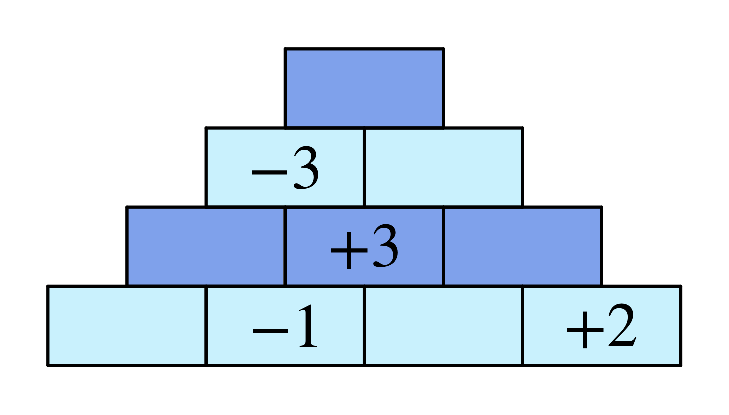
\includegraphics[width=4cm]{pyramide3_MultDivRelatifs} \end{center}
\end{minipage} \hfill%
 \begin{minipage}[c]{0.48\linewidth}
\begin{center} 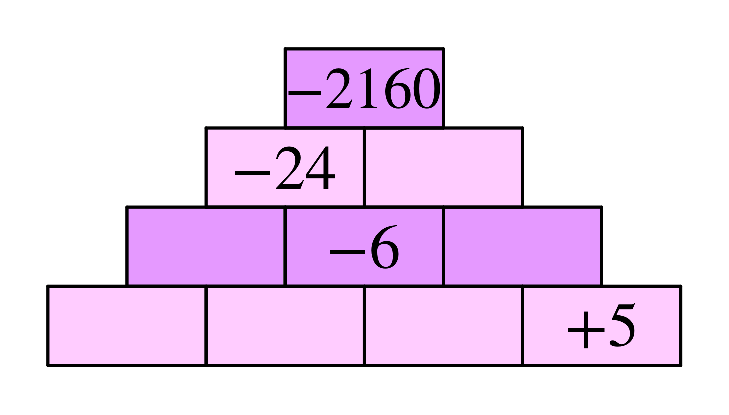
\includegraphics[width=4cm]{pyramide4_MultDivRelatifs} \end{center}  
\end{minipage} \\
\end{exercice}


\begin{exercice}
Effectue les calculs suivants en détail :
\begin{colenumerate}{2}
 \item $7 + (-6) \times (-6)$ ;
 \item $13 - (+3) \times (-4) - 8$ ;
 \item $-30 : (-9 + 15)$ ;
 \item $-3 -9 \times (-3)$ ;
 \item $-3 \times 6 \times (-2 + 8)$.
 \end{colenumerate}
\end{exercice}


\begin{exercice}
Effectue les calculs suivants en détail :
{\footnotesize
\begin{colenumerate}{2}
 \item $-22 + (13 - 5) \times (-5)$;
 \item $(-2) \times 8 + 2 \times (-20) : 4$;
 \item $-28 + (5 - 2) \times (-4)$;
 \item $7 \times (-7) + 3 \times (-25) : (-5)$;
 \item $3,2 \times (-6) + (-2,3 - 7,7)$;
 \item $150 : (-1,2 - 9 \times 3,2)$.
 \end{colenumerate}}
\end{exercice}


\begin{exercice}[Vocabulaire]
\begin{enumerate}
 \item Traduis les phrases suivantes par un calcul :
 \begin{itemize}
  \item \textcolor{A1}{La somme du produit de 4 par $-5$ et de $-6$ ;}
  \item \textcolor{H1}{Le produit de la somme de 7 et de $-8$ par la somme de 8 et de $-2$.}
  \end{itemize}  
 \item Effectue ces calculs.
 \end{enumerate}
\end{exercice}


\begin{exercice}[Vocabulaire (bis)]
Traduis les expressions mathématiques suivantes par des phrases. \\[0.2em]
Exemple : $(-2) \times 3 + 1$ se traduit par \\[0.2em]
« \textcolor{A1}{La somme du produit de $(-2)$ par 3 et de 1.} »\\
{\small
\begin{colenumerate}{2}
 \item $A = 5 \times (-7) + 3$ ;
 \item $B = 3 + 2 : (-4)$ ;
 \item $C = 7 - 4 \times (-10)$ ;
 \item $D = (2 - 3) \times (-1 - 2)$ ;
 \item $E = (1 - 7) : (2 + 5)$ ;
 \item $F = -2 +(-6) \times (6) - 9$.
 \end{colenumerate}}
\end{exercice}


\begin{exercice}
Complète le tableau suivant :
{\small
\begin{center}
\begin{tabular}{|c|c|c|c|c|c|c|}
\hline
\cellcolor{H2} $a$ & \cellcolor{H2} $b$ & \cellcolor{H2} $c$ & \cellcolor{A2} $a$ $\times$ $b$ &  \cellcolor{A2} ($-$ $a$) $\times$ $c$ &  \cellcolor{A2} $-$ ($a$ $\times$ $c$) &  \cellcolor{A2} $a$ $\times$ $b$ $\times$ $c$ \\\hline 
\cellcolor{H3} $-5$ & \cellcolor{H3} & \cellcolor{H3} $+4$ & \cellcolor{A3} & \cellcolor{A3} & \cellcolor{A3} & \cellcolor{A3} \\\hline
\cellcolor{H3} & \cellcolor{H3} & \cellcolor{H3} $+2$ & \cellcolor{A3} & \cellcolor{A3} & \cellcolor{A3} $-12$ & \cellcolor{A3} $-36$ \\\hline
 \end{tabular}
 \end{center}
 } % fin du small
\end{exercice}

\end{colonne*exercice}


\exercicesappr
\begin{colonne*exercice}
\begin{exercice}[Températures]
Pour mesurer la température, il existe plusieurs unités. Celle que nous utilisons en Suisse est le degré Celsius ($^\circ$C). Cette unité est faite de façon à ce que la température à laquelle l'eau se transforme en glace est $0^\circ$C et celle à laquelle l'eau se transforme en vapeur est $100^\circ$C. Dans cette échelle, il existe des températures négatives. \\[0.5em]
Il existe une autre unité, le Kelvin (K), dans laquelle les températures négatives n'existent pas. Pour passer de l'une à l'autre, on utilise la formule :

\begin{center} $T_\text{Kelvin} = T_\text{degrés Celsius} + 273,15$ \end{center}
       
Ainsi, $10^\circ$C correspondent à 283,15 K.
\begin{enumerate}
 \item Convertis en Kelvin les températures suivantes : $24^\circ$C ; $-3^\circ$C et $-22,7^\circ$C.
 \item Convertis en degré Celsius les températures suivantes : 127,7 K ; 276,83 K ; 204 K et 500 K.
 \item Quelle est en Kelvin la plus petite température possible ? À quelle température en degré Celsius correspond-elle ? Cette température est appelée le zéro absolu.
 \end{enumerate}
\end{exercice}


\begin{exercice}[Sur un axe gradué]
\begin{enumerate}
 \item Soit $A$ le point d'abscisse 4. Quelle peut-être l'abscisse du point $B$ sachant que la longueur du segment $[AB] = 8$ ?
 \item Soit $C$ le point d'abscisse $-3$. Quelle peut-être l'abscisse du point $D$ sachant que la longueur du segment $[CD] = 2$ ?
 \item Soit $E$ le point d'abscisse $-5$. Détermine l'abscisse de $F$ sachant que la longueur du segment $[EF] = 9$ et que l'abscisse de $F$ est inférieure à celle de $E$.
 \end{enumerate}
\end{exercice}


\begin{exercice}[Signes mystères]
Remplace les pointillés par le signe $-$ ou le signe $+$ de sorte que les égalités soient vraies :
\begin{enumerate}
 \item $\ldots \, 7 \, \ldots \, 3 = -4$ ;
 \item $\ldots \, 13 \, \ldots \, 8 = -21$ ;
 \item $\ldots \, 3,7 \, \ldots \, 8,4 = 4,7$ ;
 \item $\ldots \, 45 \, \ldots \, 72 = -27$ ;
 \item $\ldots \, 2 \, \ldots \, 7 \, \ldots \, 13 = -8$ ;
 \item $\ldots \, 1,5 \, \ldots \, 2,3 \, \ldots \, 4,9 = -5,7$ ;
 \item $\ldots \, 8 \, \ldots \, 5 \, \ldots \, 12 \, \ldots \, 2 = 13$ ;
 \item $\ldots \, 7 \, \ldots \, 14 \, \ldots \, 18 \, \ldots \, 3 = -22$.
 \end{enumerate}
\end{exercice}


\begin{exercice}[Carré magique]
Complète ce carré magique sachant qu'il contient tous les entiers de $-12$ à 12 et que les sommes des nombres de chaque ligne, de chaque colonne et de chaque diagonale sont toutes nulles :
\begin{center}
\begin{tabular}{|*5{@{}>{\vrule width0pt height\dimexpr1cm/2+1ex-.2pt\relax depth\dimexpr1cm/2-1ex-.2pt\relax\centering\arraybackslash}p{\dimexpr1cm-.4pt\relax}@{}|}}\hline
    & & 0 & 8 & \\\hline
    & & & $-11$ & 2 \\\hline
   $-9$ & $-1$ & 12 & & 3 \\\hline
   $-3$ & & $-12$ & & 9 \\\hline
   $-2$ & 11 & $-6$ & 7 & \\\hline
\end{tabular}
 \end{center}
\end{exercice}


\begin{exercice}[Triangle magique]
La somme des nombres de chaque côté du triangle est 2. Remplis les cases vides avec les nombres relatifs $(-2)$ ; $(-1)$ ; 1 ; 2 et 3, qui doivent tous être utilisés.
\begin{center} 
\includegraphics[width=3.5cm]{triangle_magique} \end{center}
\end{exercice}


\begin{exercice}[Coup de froid]
Chaque matin de la 1\up{re} semaine du mois de Février, Julie a relevé la température extérieure puis a construit le tableau suivant :
\begin{center}
\begin{tabularx}{1.07\linewidth}{|c|*{7}{>{\centering\arraybackslash}X|}} 
\hline
\cellcolor{H2} Jour & \cellcolor{H3} Lu & \cellcolor{H3} Ma & \cellcolor{H3} Me & \cellcolor{H3} Je & \cellcolor{H3} Ve & \cellcolor{H3} Sa & \cellcolor{H3} Di \\\hline
\cellcolor{A2} \small{Température (en $^\circ$C)} & \cellcolor{A3} $-4$ & \cellcolor{A3} $-2$ & \cellcolor{A3} $-1$ & \cellcolor{A3} $+1$ & \cellcolor{A3} 0 & \cellcolor{A3} $+2$ & \cellcolor{A3} $-3$ \\\hline
 \end{tabularx}
\end{center}
Calcule la moyenne des températures relevées par Julie.
\end{exercice}


\begin{exercice}
Complète les carrés magiques suivants :
\begin{enumerate}
 \item Pour l'addition :
 \vspace{.5em}
 \begin{center}
\begin{tabular}{|*3{@{}>{\vrule width0pt height\dimexpr1cm/2+1ex-.2pt\relax depth\dimexpr1cm/2-1ex-.2pt\relax\centering\arraybackslash}p{\dimexpr1cm-.4pt\relax}@{}|}}\hline
    &  $-9$ & $-2$  \\\hline
    &  $-4$ &  \\\hline
    $-6$ &  &  \\\hline
\end{tabular}
 \end{center}
 \vspace{.5em}
 \item Pour l'addition :
 \vspace{.5em}
  \begin{center}
\begin{tabular}{|*3{@{}>{\vrule width0pt height\dimexpr1.4cm/2+1ex-.2pt\relax depth\dimexpr1.4cm/2-1ex-.2pt\relax\centering\arraybackslash}p{\dimexpr1.4cm-.4pt\relax}@{}|}}\hline
 1,6 &   &  \\ \hline
 &  $-5,4$ &  \\ \hline
 $-4,4$ &  &  $-12,4$ \\ \hline
\end{tabular}
\end{center}
\vspace{.5em}
 \item Pour la multiplication :
 \vspace{.5em}
 \begin{center}
\begin{tabular}{|*3{@{}>{\vrule width0pt height\dimexpr1cm/2+1ex-.2pt\relax depth\dimexpr1cm/2-1ex-.2pt\relax\centering\arraybackslash}p{\dimexpr1cm-.4pt\relax}@{}|}}\hline
    &  36 & $-3$  \\\hline
    &  6 &   \\\hline
    $-12$ &  &  \\\hline
\end{tabular}
 \end{center}
 \end{enumerate}
\end{exercice}


\begin{exercice}
La différence $a - b$ est égale à 12.

On augmente $a$ de 3 et on diminue $b$ de 4.

Combien vaut la différence entre ces deux nouveaux nombres? 
\end{exercice}


\begin{exercice}[Le nombre $-21$...]
\begin{enumerate}
 \item Écris le nombre $-21$ comme somme de deux nombres entiers relatifs consécutifs ;
 \item Écris le nombre $-21$ comme différence de deux carrés.
 \end{enumerate}
\end{exercice}


\begin{exercice}
Recopie et complète les phrases suivantes :
\begin{enumerate}
 \item $-21$ est la moitié de \ldots \ldots ;
 \item $-21$ est le triple de \ldots \ldots ;
 \item $-21$ est l'opposé de \ldots \ldots.
 \end{enumerate}
\end{exercice}


\begin{exercice}[Choisir deux nombres]
\begin{enumerate}
 \item Trouve deux nombres relatifs dont le produit est positif et la somme est négative ;
 \item Trouve deux nombres relatifs dont le produit est négatif et la somme est positive ;
 \item Trouve deux nombres relatifs dont le produit et la somme sont positifs ;
 \item Trouve deux nombres relatifs dont le produit et la somme sont négatifs.
 \end{enumerate}
\end{exercice}


\begin{exercice}[Énigme]
Sachant que le produit deux nombres $A$ et $B$ est positif et que leur somme est négative, quels sont les signes de $A$ et de $B$ ?
\end{exercice}


\begin{exercice}[Calculatrice]
Effectue à la calculatrice les calculs suivants :
\begin{colenumerate}{2}
 \item $13\,857 \times (-253)$ ;
 \item $\dfrac{-44\,980}{8\,996 - 10\,380}$ ;
 \item $312 - 123 \times (-734)$ ;
 \item $\dfrac{-34 \times (-713)}{-68}$.
 \end{colenumerate}
\end{exercice}


\begin{exercice}[Signe]
$A$ est le produit de 24 nombres (non nuls) comportant 23 facteurs négatifs.\\[0.5em]
$B$ est le produit de 13 nombres (non nuls) comportant 11 facteurs négatifs.\\[0.5em] 
Donne, si c'est possible, le signe de :
\begin{colenumerate}{3}
 \item $A \times B$ ;
 \item $A : B$ ;
 \item $A - B$ ; 
 \item $A^{2}$ ;
 \item $A + B$.
 \end{colenumerate}           
\end{exercice}





\end{colonne*exercice}

\connaissances


\QCMautoevaluation{Pour chaque question, plusieurs réponses sont
  proposées.  Déterminer celles qui sont correctes.}

\begin{QCM}
  \begin{GroupeQCM}
    \begin{exercice}
      $(-10) + (+15) = \ldots$
      \begin{ChoixQCM}{4}
      \item $(-5)$
      \item $(-150)$
      \item $(+5)$
      \item $(-25)$
      \end{ChoixQCM}
\begin{corrige}
     \reponseQCM{a} %j'ai mis "a" partout
   \end{corrige}
    \end{exercice}
    
    
    \begin{exercice}
      (+8) + \ldots = (-5)
      \begin{ChoixQCM}{4}
      \item $(+3)$
      \item impossible
      \item $(-13)$
      \item $(-3)$
      \end{ChoixQCM}
\begin{corrige}
     \reponseQCM{a}
   \end{corrige}
    \end{exercice}
    
    
    \begin{exercice}
      $(+2,1) + (-3,9) = \ldots$
      \begin{ChoixQCM}{4}
      \item 6
      \item $-6$
      \item $-1,8$
      \item 1,8
      \end{ChoixQCM}
\begin{corrige}
     \reponseQCM{a}
   \end{corrige}
    \end{exercice}
    
    
    \begin{exercice}
      $(+7) - (-3) = \ldots$
      \begin{ChoixQCM}{4}
      \item 4
      \item 10
      \item $-4$
      \item $-10$
      \end{ChoixQCM}
\begin{corrige}
     \reponseQCM{a}
   \end{corrige}
    \end{exercice}
    
    
    \begin{exercice}
      $(-2) - \ldots = (-5)$
      \begin{ChoixQCM}{4}
      \item $(+3)$
      \item $(-7)$
      \item $(+7)$
      \item $(-3)$
      \end{ChoixQCM}
\begin{corrige}
     \reponseQCM{a}
   \end{corrige}
    \end{exercice}
    
    
    \begin{exercice}
      $1,3 - (-2,4) = \ldots$
      \begin{ChoixQCM}{4}
      \item $-1,1$
      \item $1,1$
      \item $3,7$
      \item $-3,7$
      \end{ChoixQCM}
\begin{corrige}
     \reponseQCM{a}
   \end{corrige}
    \end{exercice}
    
    
    \begin{exercice}
      $-7 \times (-3) = \ldots$
      \begin{ChoixQCM}{4}
      \item $-10$
      \item $-21$
      \item 10
      \item 21
      \end{ChoixQCM}
\begin{corrige}
     \reponseQCM{a}
   \end{corrige}
    \end{exercice}
    
    
    \begin{exercice}
      $4 \times (-3) = \ldots$
      \begin{ChoixQCM}{4}
      \item 1
      \item $-12$
      \item $-7$
      \item 12
      \end{ChoixQCM}
\begin{corrige}
     \reponseQCM{a}
   \end{corrige}
    \end{exercice}
    
    
    \begin{exercice}
      $-15 : (-5) = \ldots$
      \begin{ChoixQCM}{4}
      \item $(-15) : (-5)$
      \item $-3$
      \item $15 : 5$
      \item $3$
      \end{ChoixQCM}
\begin{corrige}
     \reponseQCM{a}
   \end{corrige}
    \end{exercice}
    
    
    \begin{exercice}
      $4 \times (-4) = \ldots$
      \begin{ChoixQCM}{4}
      \item 0
      \item $-8$
      \item 16
      \item $-16$
      \end{ChoixQCM}
\begin{corrige}
     \reponseQCM{a}
   \end{corrige}
    \end{exercice}

    
    \begin{exercice}
      Le produit de l'opposé de $-6$ par l'opposé de 7 vaut \ldots
      \begin{ChoixQCM}{4}
      \item 42
      \item $-42$
      \item $-1$
      \item $6 : (-7)$
      \end{ChoixQCM}
\begin{corrige}
     \reponseQCM{a}
   \end{corrige}
    \end{exercice}
    
    
    \begin{exercice}
      $-6 + 6 \times (-10) = \ldots$
      \begin{ChoixQCM}{4}
      \item 0
      \item 120
      \item 66
      \item $-66$
      \end{ChoixQCM}
\begin{corrige}
     \reponseQCM{a}
   \end{corrige}
    \end{exercice}


    \begin{exercice}
      Le produit de 108 facteurs égaux à $-1$ est égal à \ldots
      \begin{ChoixQCM}{4}
      \item $-108$
      \item 0
      \item 1
      \item $-1$
      \end{ChoixQCM}
\begin{corrige}
     \reponseQCM{a}
   \end{corrige}
    \end{exercice}
    
\end{GroupeQCM}
\end{QCM}

  


\TravauxPratiques % pour nous "travailler en groupe"

\begin{TP}[Morphing]

Le \textbf{morphing} ou \textbf{morphage} est un des effets spéciaux applicables à un dessin. Il consiste à fabriquer une animation qui transforme de la façon la plus naturelle et la plus fluide possible un dessin initial vers un dessin final. 

\partie{Construction d'une image}
\begin{enumerate}
 \item Construisez un repère (chaque élève du groupe le fait sur son cahier).\\[0.5em] \label{MultDivRel_TP1}
Placez les points suivants dans le repère :\\[0.5em]
\begin{center}
\renewcommand*\tabularxcolumn[1]{>{\centering\arraybackslash}m{#1}}
\begin{ttableau}{0.8\linewidth}{4}
$A(0 ; 1)$ & $B(-4 ; 1)$ & $C(0 ; 5)$ & $D(0 ; -1)$ \\
$E(-3 ; -1)$ & $F(-2 ; -3)$ & $G(3 ; -3)$ & $H(4 ; -1)$ \\
$I(3 ; -1)$ & $J(3 ; 3)$ & $K(1 ; 2)$ & $L(3 ; 1)$ \\
 \end{ttableau}
\end{center}
\vspace{0.3cm}
Reliez à la règle les points dans l'ordre alphabétique de $A$ jusqu'à $L$ puis tracez le segment $[DI]$.
 \item Cette figure tient dans un carré. Construisez ce carré en rouge.
 \end{enumerate}
        
\partie{Transformation} \label{MultDivRel_TP2}
Pour cette partie, le travail peut être réparti entre les différents membres du groupe. Voici plusieurs transformations subies par les coordonnées des points :
\begin{itemize}
 \item On échange son abscisse et son ordonnée. On obtient $A_1$, $B_1$ \ldots ;
 \item On double son abscisse. On obtient $A_2$, $B_2$ \ldots ;
 \item On double son ordonnée. On obtient $A_3$, $B_3$ \ldots ;
 \item On double son abscisse et son ordonnée. On obtient $A_4$, $B_4$ \ldots ;
 \item On ajoute 4 à son abscisse et $-3$ à son ordonnée. On obtient $A_5$, $B_5$ \ldots.
 \end{itemize}
\begin{enumerate}
 \setcounter{enumi}{2}
 \item Pour chacune de ces transformations, indiquez les nouvelles coordonnées de chaque point puis construisez la figure dans un nouveau repère et enfin écrivez une phrase pour indiquer ce qu'est devenu le carré rouge.
 \end{enumerate}
        
\partie{Chacun sa figure}
\begin{enumerate}
 \setcounter{enumi}{3}
 \item Construisez la figure de votre choix dans un repère (15 points au maximum). Faites bien attention à ce que tous les points aient des coordonnées entières. À partir du dessin, remplissez un tableau de points comme à la question \ref{MultDivRel_TP1}.
 \item Donnez ce tableau à un autre groupe pour qu'il réalise la figure puis une transformation de votre choix parmi celles de la partie \ref{MultDivRel_TP2}.
 \end{enumerate}

\end{TP}

%%%%%%%%%%%%%%%%%%%%%%%%%%%%%%%%%%%%%%%%%%%%%%%%%%%%%%%%%%%%%%%%%%%%%%
%%%%%%%%%%%%%%%%%%%%%%%%%%%%%%%%%%%
%%%%%%%%%%%%%%%%%%%%%%%%%%%%%%%%%%%
%MiseEnPage
%%%%%%%%%%%%%%%%%%%%%%%%%%%%%%%%%%%
\newpage
%%%%%%%%%%%%%%%%%%%%%%%%%%%%%%%%%%%
%%%%%%%%%%%%%%%%%%%%%%%%%%%%%%%%%%%



\begin{TP}[Le bon produit]

\partie{La construction du jeu}
\begin{enumerate}
 \item Avec du papier épais ou du carton, fabriquez  66 cartes à jouer.
 \item Au stylo bleu, fabriquez les 38 cartes « facteur » :
 \begin{itemize}
  \item Deux portent le nombre 0 ;
  \item Trois exemplaires pour chacun des nombres : $-9$ ; $-6$ ; $-4$ ; $-3$ ; $-2$ ; $-1$ ; 1 ; 2 ; 3 ; 4 ; 6 et 9.
  \end{itemize}
\underline{Remarque} : Soulignez les 6 et les 9 pour éviter de les confondre.
 \item Au stylo rouge, fabriquez les 28 cartes « produit » :
 \begin{itemize} 
  \item Deux portent le nombre 0 ;
  \item Les autres sont toutes différentes et portent les nombres : $-54$ ; $-36$ ; $-27$ ; $-24$ ; $-18$ ; $-16$ ; $-12$ ; $-9$ ; $-8$ ; 6 ; $-4$ ; $-3$ ; $-2$ ; 2 ; 3 ; 4 ; 6 ; 8 ; 9 ; 12 ; 16 ; 18 ; 24 ; 27 ; 36 et 54.
  \end{itemize}
 \end{enumerate}

\partie{Les règles du jeu} 
Chaque joueur reçoit six cartes « facteur » puis pioche une carte « produit ». Celui qui a le plus grand nombre joue en premier (en cas d'égalité, les joueurs ex-aequo piochent une deuxième carte produit). On tourne ensuite dans le sens des aiguilles d'une montre.\\[0.5em]
Les cartes « produit » piochées sont posées face visible. On complète de façon à en avoir 10 en tout sur la table.\\[0.5em]
Le joueur dont c'est le tour pioche une carte « produit » et la pose sur la table avec les autres.\\[0.5em]
Si, avec deux de ses cartes facteurs, il peut obtenir un des produits visibles, il écarte les trois cartes (les deux cartes « facteur » et la carte « produit »).\\[0.5em]
S'il ne peut pas, il pioche deux cartes « facteur » et regarde à nouveau s'il peut obtenir un produit.\\[0.5em]
S'il propose une combinaison et qu'il a fait une erreur de calcul, il pioche également deux cartes « facteur ».\\[0.5em]
C'est alors au tour du joueur suivant.\\[0.5em]
Lorsqu'un joueur a écarté toutes ses cartes « facteur », il a gagné.

\end{TP}

%%%%%%%%%%%%%%%%%%%%%%%%%%%%%%%%%%%
%%%%%%%%%%%%%%%%%%%%%%%%%%%%%%%%%%%
%MiseEnPage
%%%%%%%%%%%%%%%%%%%%%%%%%%%%%%%%%%%
\vfill
%%%%%%%%%%%%%%%%%%%%%%%%%%%%%%%%%%%
%%%%%%%%%%%%%%%%%%%%%%%%%%%%%%%%%%%



\pagebreak

\recreation
\begin{enigme}[Le compte est bon]

Avec les nombres proposés, retrouve les résultats annoncés ! \\[0.5em]
Tu ne peux utiliser chaque nombre qu'une seule fois. Toutes les opérations sont autorisées.\\[0.5em]
Avec $-3$ ; $-5$ ; 25 ; $-100$ et 7, trouve $-650$.\\[0.5em]
Avec $-7$ ; $-25$ ; 10 ; $-8$ et $-75$, trouve 730.

\end{enigme} 



